%% LyX 2.3.6 created this file.  For more info, see http://www.lyx.org/.
%% Do not edit unless you really know what you are doing.
\documentclass[10pt]{article}
\usepackage{helvet}
\renewcommand{\familydefault}{\sfdefault}
\usepackage[T1]{fontenc}
\usepackage[utf8]{inputenc}
\usepackage[a4paper]{geometry}
\geometry{verbose,tmargin=2cm,bmargin=4cm,lmargin=2cm,rmargin=2cm}
\usepackage{fancyhdr}
\pagestyle{fancy}
\setlength{\parskip}{6pt}
\setlength{\parindent}{0pt}
\usepackage{tcolorbox}
\usepackage{amsmath}
\usepackage{amsthm}
\usepackage{amssymb}
\usepackage{todonotes}
\usepackage{graphicx}
\usepackage[backend=biber,maxbibnames=99]{biblatex}
\addbibresource{main.bib}

\makeatletter

%%%%%%%%%%%%%%%%%%%%%%%%%%%%%% LyX specific LaTeX commands.
%% A simple dot to overcome graphicx limitations
\newcommand{\lyxdot}{.}


%%%%%%%%%%%%%%%%%%%%%%%%%%%%%% User specified LaTeX commands.
\usepackage{tcolorbox}
\usepackage{amsthm}
\usepackage{lastpage}
\usepackage{fancyhdr}
\usepackage{accents}
\usepackage{titlesec}
\usepackage{marginnote}
\usepackage{titlesec}
\titleformat{\section}[block]{\normalfont\bfseries}{}{0em}{}


\usepackage{enumitem}
\usepackage{comment}
\setlist{nolistsep}

\usepackage{tcolorbox}
\definecolor{light-blue}{cmyk}{0.24, 0.12, 0.0, 0.04, 1.00}
\titlespacing\section{0pt}{0pt}{0pt}
\titlespacing\subsection{0pt}{0pt}{0pt}
\titlespacing\subsubsection{0pt}{0pt}{0pt}

\setlength{\headheight}{40pt}

\makeatother

\begin{document}
\lhead{Neimhin Robinson Gunning} \rhead{CS7CS4 Final Assignment}

\section{DublinBike Usage}
Here we investigate the impact of the coronavirus pandemic on
DublinBike usage, by comparing forecasts base on pre-pandemic data
with the recorded usage during and after the pandemic period.

The first unilateral government guidelines in Ireland regarding
mitigation of viral spread were issued and came into affect on
the 12th of March 2020 \cite{leahy2020coronavirus}. For the purposes of this investigation
we regard this date as the start of the pandemic era. This is
admittedly somewhat arbitrary; cases of Covid-19 were recorded earlier
in Feb 2020.
We consider 28th February 2022 as the end of the pandemic in Ireland
because on this date almost public health restrictions were lifted \cite{molony2022almost}.
Again this is somewhat arbitrary.

Reportedly:
``Data released by Dublin City Council to this website shows that usage last year was still around 1.8 million trips down from pre-pandemic levels — with 2,001,810 trips by users in 2022 compared to 3,816,652 in 2019.'' \cite{ginty2023dublinbikes}.

\subsection{Engineering a ``usage'' feature}
The dublin bike dataset used for this analysis consists
of snapshots of station occupancy at five-minute intervals.
Because of this it is not possible to determine from the
dataset the exact number of times bikes have been
returned to or taken from a station.
We can look at the difference in bike occupancy at the
beginning and end of a five-minute interval to establish
a {\em lower-bound} on the number of interactions with
the station, but it is possible for there to have been
more interactions (returns or borrowings) than this difference, i.e. the difference lies.
For instance, it may be that a bike station has 10 bikes at time $t$
and 10 bikes at time $t+5\text{m}$, but that in fact 5 bikes were
borrowed {\em and} 5 bikes were deposited.

But, we can detect such cases, because the dataset also includes a
\textsc{last updated} field. If the occupancy is not changed, but 
the time of last update is between the start and end of the interval,
then we know that there were at least 2 interactions with the bike station.
In such cases there can only have been an even number of interactions, ${2,4,6,\ldots}$, and we
can assume a geometric distribution over these possibilities.
Let $g_{\text{missed}}$ be the true probability distribution over these possibilities.

We compute the \textsc{has changed} column by $$\textsc{has changed}_i = 
\begin{cases} 
1 & \text{if } \textsc{LAST UPDATED}_i > \textsc{TIME}_{i - 1} \\
0 & \text{otherwise}
\end{cases}
$$ and then $$\textsc{missed change}_i = \textsc{has changed}_i \land (\textsc{diff}_i = 0)$$

Considering occupancy data spanning 1st Jan 2020 to 1st Apr 2020, \textsc{missed change} is true
about for about 37\% ($828673/2228278$) of the intervals.
We must also remember that there are cases where \textsc{available bikes} has changed, but the difference in occupancy does not reflect the true number
of interactions. There is no way to detect these cases.

But is it possible to get more information about this
distribution from the data?
Yes, if we can estimate the rate of bike removals.

Something we can estimate without caveats is the distribution of time since the last update.


\subsubsection{Usage over time}
% LOWER BOUND TAKE OUTS
% note that the 2018 and 2023 years are incomplete
% YEAR  LOWER BOUND JOURNEYS
% 2018             2603824.0
% 2019             5721975.0
% 2020             5194359.0
% 2021             5308306.0
% 2022             1074247.0
% 2023             1062018.0

% YEAR           NUM SAMPLES
% 2018               4937925
% 2019              10691784
% 2020              10896643
% 2021              11157202
% 2022               1982257
% 2023               1972740

% YEAR   AVAILABLE BIKES DIFF RELU
% 2018                     1094039
% 2019                     2334214
% 2020                     1358085
% 2021                     1357736
% 2022                     9564400
% 2023                     9860396

% irishcycle.com report
% YEAR          NUM JOURNEYS
% 
% 2019               3816652
%
%
% 2022 	             2001810

\subsubsection{A `usage' feature based on \textsc{last updated}}
Because of all the severe caveats with the difference based `usage' features
we seek an alternative based on the \textsc{last updated} column.
First, we assume variable, the arrival rate, which changes over time.
The arrival rate is the expected number of uses of a bike station per minute.
We can estimate the arrival based on the \textsc{last updated} variable.

For each snapshot the station's state we can calculate the amount of time since the last update, $\Delta t$.
Absent of other contextual evidence, the inverse of this is the best estimate of the arrival rate, $\lambda_{[\text{user/minute}]} = \frac{1}{\Delta t}$.
Since samples are taken every 5 minutes, we can then multiply the arrival rate by 5 minutes 
to estimate the number of interactions with the bike station,
$\hat{\text{\#interactions}} = 5 \times \lambda$.
This calculation yields the unfortunate result where time intervals that are
known to have no interactions will have a small non-zero number of estimated interactions.

We can further adjust the estimation of the arrival rate by aggregating across more samples, e.g.
for an hour interval, take the average of \textsc{last updated}, and use $\hat{\text{\#interactions}} = 60 \times \lambda$.
Or, for a particular time of day, aggregate across multiple days, etc.

There is a problem with this approach due to an apparent bug in how the dataset was created.
There are cases where the snapshot seemingly misreports \textsc{last updated}. In the below snippet from
the second row shows that there was an update at 22:13, but the snapshot for 22:15 indicates the last update was at 22:08.
This is a contradiction.
%      STATION ID                TIME        LAST UPDATED
%               2 2018-08-01 22:15:03 2018-08-01 22:08:30
%               2 2018-08-01 22:20:01 2018-08-01 22:13:50
%               2 2018-08-01 22:25:01 2018-08-01 22:20:24

We have intentionally avoided the use of lagged features, e.g. to predict the usage at time $t$, aggregate data from times $t-n,t-2n,\ldots$, for the reason
that such features would themselves have to be estimated when making predictions outside the pre-pandemic era.
This would result in wilder and less interpretable predictions.

In summary, there is no way to accurately derive a semantically precise usage metric from the
dataset, such as the number of journeys, or the amount of rental time.
We must settle for a proxy usage metric. We define our pseudo-usage metric based the global
change in the number of available bikes.
First we thin all of the data, keeping only snapshots taken at intervals of 30 minutes.
We do this because a significant portion of the dataset uses only 30 minute, rather than 5 minute, snapshots.
It is only the pandemic and post-pandemic era data that have this sampling style.
Since the purpose of the analysis is to compare the different eras,
we thin the data such that the sampling style is consistent throughout the dataset.

We then group samples by time interval and sum \text{AVAILABLE BIKES} for all stations, to get the global number
of available bikes $g_t$ at each point in time.
Our usage statistic $u_{\text{30m}}$ is then the absolute value of the difference between $g_t$ at subsequent intervals: $u_{\text{30m}^t}=|g_t-g_{t-\text{30m}}|$.
For analysis, we also use an aggregated version of this metric, summing $g_t$ over the interval of a day or a month,
$$ u_\text{M}=\sum_{t\in M}g_t $$.

The input features for forecasting are:
\begin{itemize}
    \item \textsc{timestamp}: The unix epoch time of the sample rounded to the nearest thirty minutes.
    \item \textsc{workday}: Whether or not the sample was taken on a workday. Set to 0 for non-workdays, including weekends, bank holidays, and national holidays, 1 for workdays.
    \item \textsc{interval}: A one-hot encoding of the time of day. With sample frequency of 30 minutes there are 48 intervals, and thus this one-hot vector has length 48.
\end{itemize}

\subsection{Forecasting Usage}
To forecast (counterfactually), DublinBike usage in the pandemic and post-pandemic eras we isolate the
pre-pandemic DublinBike data for model development and evaluation.

We notice that the distributions for working days and non-working days are obviously different, and thus
we use a baseline predictor based on two subsets of the data, working days and non-working days.
This `split baseline' uses the mean pseudo-usage of both subsets for predictions:
$$\hat{u}_i = 
\begin{cases} 
E[u|\text{workday}] & \text{if workday} \\
E[u|\lnot\text{workday}] & \text{if not workday}
\end{cases}
$$

We use a pair of Lasso linear regression models, one trained on the `workday' subset, and the other
trained on the `non-workday' subset. We call this the `dual lasso' predictor.
We found that a single lasso model performed much worse than the `split baseline'.

Each lasso model has $48+1+1=50$ trainable parameters we call $\theta$.
The input features are arranged in a vector of length 51, with one dummy feature that is always 1: $$x=[1,\text{timestamp},\ldots\text{interval one-hot}]$$
The model for prediction is then $\hat{y}(x) = \theta^{\intercal}x$.
The model for prediction of the dual lasso model is therefore $$
\begin{cases}
    \hat{y}_{\text{workday}}(x_t)     & \text{if } t \in \text{workdays} \\
    \hat{y}_{\text{non-workday}}(x_t) & \text{if } t\notin \text{workdays}
\end{cases}    
$$.

This model inherently enforces a prediction of approximately linear growth rate of usage,
but accounts for the fact that there are
different numbers of holidays for different time intervals.
The pre-pandemic era data spans less than 2 years which is
not enough data to detect non-linear growth rate year-on-year,
so we decided to choose a model which inherently can not predict exponential or geometric growth.

The hyperparameter $\alpha$ is selected independently for each of the `dual lasso' submodels.
5-fold cross-validation, without shuffling of data, is used. The reason not to shuffle the data
is that we are trying to forecast usage well outside the domain of the training data.
By not shuffling we ensure that a larger portion of the test data is further outside the time-domain
seen in the training data, meaning we are evaluating the model's ability to generalize to new time-intervals.

% Comparing dual lasso model to split baseline.
% workday mean 20.49938841540404
% non workday mean 9.810360736411969
% dual model mse: 977.0018326489687
% baseline model mse: 1166.640512328726


\subsection{Impact of Covid on Pandemic and Post-Pandemic Era}

The dual lasso model is trained to predict pseudo-usage at each 30 minute interval, but for
summary analysis we group the predictions by month and take the sum, comparing to the true data processed in the same way.
% TODO DUBIOUS
The reason we didn't train the model to predict monthly usage directly is primarily to account for the significant amount of missing data
in the dataset. This missing data means that some months have many fewer samples than others. But our model makes the same number of
predictions as there are true samples, such that when the data are aggregated over a month the comparison is fair.
If we had trained the model
to predict the monthly usage directly there would be more work to do to make sure the comparison is fair.
Secondly, the finer granularity of predictions gives greater flexibility in how the predictions are then aggregated for comparison.

The dual lasso model's predictions for the pandemic and post-pandemic eras are presented in Figure \ref{fig:dual-lasso-forecast}.
The dual lasso model essentially predicts a slow decrease in DublinBike usage, whereas in fact
there is a sharp decrease in usage at the start of the pandemic.
The dual lasso model predicts there would have been greater usage in the post-pandemic era than has actually
transpired, but the difference is less than for the pandemic era. The monthly predictions are compared to true monthly usage in Figure \ref{fig:dual-lasso-forecast}.
Notice there is a large spike in pseudo-usage in the middle of the pandemic era.
It is not clear whether this spike is from natural usage or another cause.
It is possible the spike is due to bikes being replaced/repaired/removed by the managing authority more frequently during that period.
The pseudo-usage metric is sensitive to such events, which do not constitute actual usage.

\begin{figure}
    \centering
    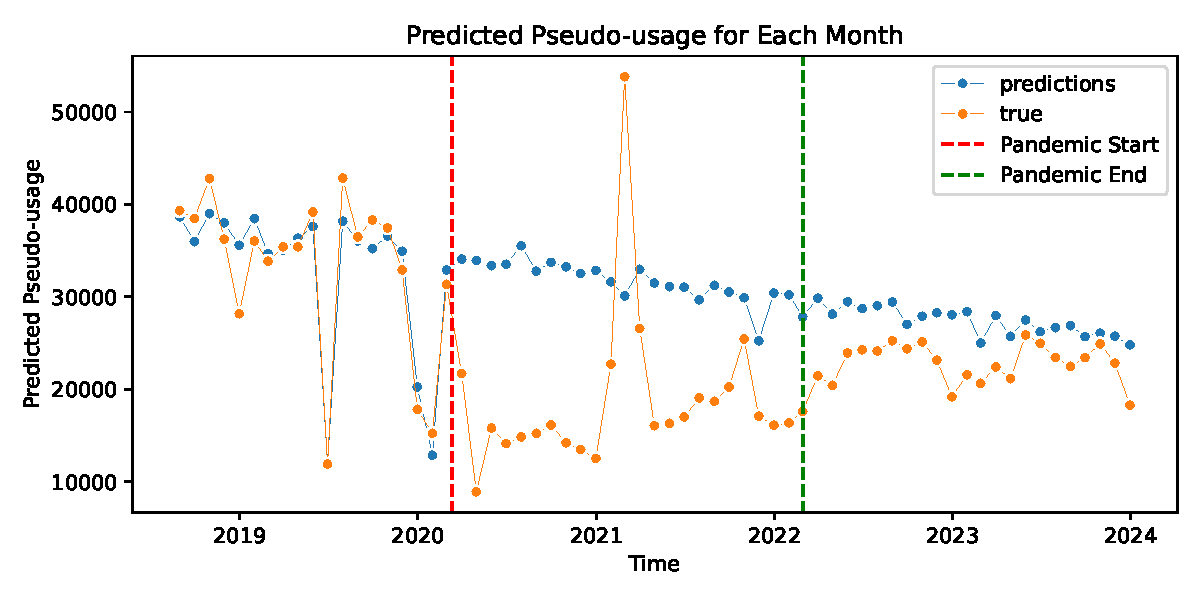
\includegraphics[width=\textwidth]{merged-all-30min.csv.d/prediction_all.csv.d/predicted-usage-month.pdf}
    \caption{Predicted vs True DublinBike Pseudo-usage, for pandemic, pre-pandemic, and post-pandemic eras. Predictions given by `dual lasso' model.}
    \label{fig:dual-lasso-forecast}
\end{figure}


% \begin{figure}[ht]
%     \centering
%     \includegraphics[width=\textwidth]{path/to/your/image.png}
%     \caption{Your descriptive caption goes here.}
%     \label{fig:your_label}
% \end{figure}

% Mean Month Difference Pre-Pandemic Era: 87.34628997389288
% Mean Month Difference Pandemic Era: -17190.651967500882
% Mean Month Difference Pandemic Era: -13456.005450214061

\begin{tabular}{l r r}
    \centering
    & dual lasso & split baseline \\
    Mean Month Difference Pre-Pandemic Era & 47 & 87 \\
    Mean Month Difference Pandemic Era   & -12989 & -17191 \\
    Mean Month Difference Pandemic Era   & -4517 & -13456 \\
\end{tabular}
% mean error pandemic era: -13051.524022983676
% mean error post pandemic era: -4645.458425274869

\section{Short Questions}
\subsection{(i)}
What is an ROC curve?

The name Receiver Operating Characteristic (ROC) is not very enlightening as to what an ROC curve is.

Often, a binary classifier consists of a function $c:X\rightarrow [0,1]$ which maps an input $x\in X$ to a the
probability that $x$ belongs to either of the classes. We can use this probability to make
a more concrete classification decision by selecting a threshold $\alpha$. For example:
\begin{equation}
\hat y(x)=
    \begin{cases}
        1 & \text{if } c(x) > \alpha, \\
        0 & \text{otherwise}
    \end{cases}
\end{equation}
Our choice of $\alpha$ changes the ultimate classification decisions.
For each choice of $\alpha$ we can calculate the True Positive Rate and False Positive Rate
of the classifier on a test data set, therefore we implicitly have a function $f:[0,1]\rightarrow \mathbb{R}^2$.
An ROC curve is a plot of the output values of this function $f$, i.e. the ROC plot generally does not
encode $\alpha$, only the output points $(\text{FPR},\text{TPR})$, so we
visualise the function $f$ as if it were a function $g:\text{FPR}\rightarrow \text{TPR}$.

\begin{equation}
    \begin{aligned}
        \text{TPR} & = \frac{\text{TP}}{\text{P}} & & \text{FPR} & = \frac{\text{FP}}{\text{N}}
    \end{aligned}
\end{equation}

The ROC curve $g$ will be monotone increasing from $0$ to $1$, but not smooth.
The `steps'
in an ROC curve occur where a small change in $\alpha$ result
in a change in classification of a single data point.

\textbf{How can it be used to evaluate the performance of a classifier?}

If the test set is fair then a `coin-flip' classifier, that just makes a random
classification for each input, will have an ROC curve approximating the line from $(0,0)$ to $(1,1)$,
with more data points giving a closer approximation. In this way the ROC curve lets you
implicitly compare a binary classifier to a `coin-flip` classifier.

In general a classifier is better if the area under the ROC curve is greater, where the maximum area is 1.
Being reductionist, this means that a classifier is better if it's ROC curve gets closer to the point the $(0,1)$.

\textbf{Why would you use an ROC curve instead of a classification accuracy metric?}
If the cost of different types of errors (false positive, false negative) are significantly
different for the particular use-case, or if the dataset is imbalanced,
then an ROC curve can be more illuminating than a reductionist accuracy metric
for evaluating whether specific requirements are being met, and it can be used to
search for the threshold $\alpha$ which balances the requirements of the task most appropriately.

\subsection{(ii)}
Linear regression will give inaccurate predictions when the target values are
not linearly correlated the input features.
For example if the target output is strongly correlated to the distance
of the input features from some point, i.e. there is a circular/spherical pattern,
then a linear regression will likely give poor predictions for a large
proportion of the data. Depending on the type of non-linearity between the
inputs and outputs it may be possible to augment the input features, e.g. by taking polynomial
combinations of the input features, such that the targets do become
linearly correlated with some subset of the augmented input features.
If this type of feature engineering doesn't work then a different model
that can handle non-linearity, such as a k-NN regression model,
could be used instead.

Linear regression can be sensitive to outliers,
where I define an outlier to be a datapoint which was generated
by some process distinct from expected process, i.e. a typo,
a faulty sensor.

\includegraphics{fig/outlier_example_linear_regression.pdf}

\subsection{(iii)}

\bigskip{}
\printbibliography
\end{document}
